\documentclass[11pt]{article}
\usepackage[margin=1in]{geometry}
\usepackage{amsmath,amssymb,amsthm,booktabs,graphicx,hyperref,array,microtype}
\usepackage{xcolor}
\hypersetup{colorlinks=true,linkcolor=blue!50!black,urlcolor=blue!50!black,citecolor=blue!50!black}
\newcommand{\NFib}{99}
\newcommand{\NSqD}{105}
\newcommand{\NSqW}{64}
\newcommand{\FibQ}{201}
\newcommand{\SqDQ}{85}
\newcommand{\SqWQ}{45}
\newcommand{\FibSmallMoves}{141}
\newcommand{\FibSmallPaths}{28}
\newcommand{\FibMaxDeg}{10}
\newcommand{\NAccRef}{607409}
\newcommand{\NAdv}{7409}
\newcommand{\NRad}{52000}
\newcommand{\NStates}{111}
\newcommand{\NCrit}{1000000}
\newcommand{\VerSha}{4356095c0527d611}
\newcommand{\FibItersMax}{7392}
\newcommand{\FibItersMean}{2595.89}
\newcommand{\SqDItersMax}{210}
\newcommand{\SqWItersMax}{355}
\newcommand{\FibSlope}{8.1}
\newcommand{\FibNoRec}{38}
\newcommand{\SqDSlope}{1.7}
\newcommand{\SqDNoRec}{87}
\newcommand{\SqWSlope}{3.4}
\newcommand{\SqWNoRec}{61}
\newcommand{\CFiboIConst}{9}
\newcommand{\CFiboILocal}{14}
\newcommand{\CFiboIAlgstate}{15}
\newcommand{\CFiboIField}{51}
\newcommand{\CFiboITarget}{0}
\newcommand{\CFiboIUnexplained}{10}
\newcommand{\CSquaTConst}{23}
\newcommand{\CSquaTLocal}{27}
\newcommand{\CSquaTAlgstate}{37}
\newcommand{\CSquaTField}{18}
\newcommand{\CSquaTTarget}{0}
\newcommand{\CSquaTUnexplained}{0}
\newcommand{\CSquaRConst}{16}
\newcommand{\CSquaRLocal}{22}
\newcommand{\CSquaRAlgstate}{23}
\newcommand{\CSquaRField}{3}
\newcommand{\CSquaRTarget}{0}
\newcommand{\CSquaRUnexplained}{0}

\newtheorem{theorem}{Theorem}
\newtheorem{proposition}[theorem]{Proposition}
\newtheorem{lemma}[theorem]{Lemma}
\newtheorem{corollary}[theorem]{Corollary}
\theoremstyle{definition}
\newtheorem{definition}[theorem]{Definition}
\theoremstyle{remark}
\newtheorem{remark}[theorem]{Remark}
\newcommand{\Q}{\mathbb{Q}}
\DeclareMathOperator{\isqrt}{isqrt}
\title{\textbf{UNNS-U2-FP-R3}\\[2pt]\large Algebraic Parameter Recovery and the Generative Knowledge Audit}
\author{UNNS Research Collective}
\date{Version v001 \quad (addendum to UNNS-U2-FP-SYM v001; that package, UNNS-U2-FP v001, U2-SQ and all earlier releases are unchanged)}
\begin{document}
\maketitle
\begin{abstract}
\noindent
The Fibonacci selector of UNNS-U2-FP-SYM recovered the parameters of its routes by bisection on a floor-based function. This addendum (i)~states the recovery rule precisely as \emph{R3$'$, fixed algebraic-monotone recovery}, and replaces the floor function by the exact algebraic function $\alpha_\varepsilon(t)=(\sqrt{5t^2+4\varepsilon}-t)/2$, with an exact continuous monotonicity certificate for all \NStates{} state functions and a sign-safe exact comparison of expressions $P+Q\sqrt D$; (ii)~re-implements the selector with these comparisons, an explicit membership test, explicit fixed-modulus dispatch and refusal of non-Fibonacci inputs, and records the recovery work separately from graph moves; and (iii)~introduces a \emph{Generative Knowledge Audit}: every route label of the Fibonacci selector and of both square selectors is classified by what it needs (a constant, a function of the current state, or recovery of route-start parameters). Result: only \FibNoRec{} of \NFib{} Fibonacci labels, against \SqDNoRec{} of \NSqD{} and \SqWNoRec{} of \NSqW{} for the two square selectors, are computable from the current state with a fixed-order root; the Fibonacci selector needs, in addition, the Cassini quadratic $5x^2\pm4=L_k^2$ and, for ten labels, half-index Fibonacci values. All three selectors can compute their target before moving. We therefore read the Fibonacci result as autonomous bounded-route generation under a restricted arithmetic selector, not generation from graph structure alone. Prime generation is not addressed; the audit defines what a prime selector would have to supply.
\end{abstract}

\section{Scope and evidence levels}
This is a separate research addendum. It re-uses, unchanged, the route certificates of UNNS-U2-FP-SYM (file \texttt{class\_certificates.json}, hash in the README) and the frozen square selectors of UNNS-U2-SQ. Three kinds of statement are kept apart.
\begin{itemize}\setlength\itemsep{1pt}
\item \emph{Certified exactly}: finite polynomial identities and coefficient-sign tests (SymPy, no proof assistant), and exact integer decision procedures.
\item \emph{Verified at sample points}: statements established by exact rational interpolation at $26$ sample points per route class and checked at all of them. These are not identities for all inputs. The audit categories below are of this kind.
\item \emph{Tested}: exhaustive or randomised runs of the implemented selectors.
\end{itemize}
Throughout, ``not found'' means not found in the stated vocabulary; it is never a necessity claim.

\section{R3$'$: fixed algebraic-monotone recovery}
The restricted-selector Definition~2.1 of UNNS-U2-FP is preserved as written. We add the following \emph{explicit clarification of its recovery clause}; it extends, and is not claimed to be implied by, a polynomial-only reading.

\begin{definition}[R3$'$]\label{def:r3}
A selector may recover an integer parameter $t$ from its current state $x$ by inverting a predeclared strictly monotone algebraic function $x=G_q(t)$, where $q$ is its finite control state, provided that: (a)~$G_q$ is specified independently of the input; (b)~its strict monotonicity, hence uniqueness of the preimage, is certified on the stated domain; (c)~all comparisons are exact, including comparisons involving radicals; (d)~inversion is a finite terminating arithmetic procedure that may use an input-dependent number of operations; (e)~no candidate sequence terms, graph paths or external targets are searched.
\end{definition}

\paragraph{Authorized primitives and their charge.} Addition, subtraction, multiplication; exact division by constants; comparison; integer square root $\isqrt$; residue $x\bmod m$ for a fixed modulus $m$ (\emph{fixed-modulus dispatch}); and the exact radical sign test of Section~\ref{sec:radical}. The verifier charges bisection iterations, exact comparisons, big-integer multiplications and square roots per input, separately from graph moves. Fixed-modulus dispatch and the membership test are authorized but must be listed in the knowledge ledger (Section~\ref{sec:ledger}).

\paragraph{What changes about uniform cost.} Because inversion may take an input-dependent number of operations, a selector under R3$'$ is finite-control but \emph{not} a uniformly bounded straight-line program. R2 (bounded programs) therefore applies to label evaluation after recovery, and recovery is charged separately. A polynomial-only reading of R3 is not satisfied by the Fibonacci selector; whether it can be (with another parametrisation) is open.

\section{Exact comparison of $P+Q\sqrt D$}\label{sec:radical}
\begin{lemma}[sign rule]\label{lem:sign}
For integers $P,Q$ and $D\ge0$: if $Q=0$ or $D=0$ the sign is $\operatorname{sgn}P$; if $P=0$ it is $\operatorname{sgn}Q$; if $\operatorname{sgn}P=\operatorname{sgn}Q$ it is that sign; otherwise it is $\operatorname{sgn}P$ if $P^2>Q^2D$, $\operatorname{sgn}Q$ if $P^2<Q^2D$, and $0$ if equal.
\end{lemma}
\begin{proof}
In the last case $P$ and $Q\sqrt D$ have opposite signs, so the sign of the sum is that of the larger absolute value, and $|P|\gtrless|Q|\sqrt D\iff P^2\gtrless Q^2D$ because both sides are non-negative. Squaring is applied only after the sign conditions have been tested.
\end{proof}
For a state function $G(t)=p_0(t)+p_1(t)\alpha_\varepsilon(t)$ with $p_0=P_0/d_0$, $p_1=P_1/d_1$ ($P_j$ integer polynomials) and an integer $x$,
\[
2d_0d_1\bigl(G(t)-x\bigr)=\underbrace{2d_1P_0(t)-d_0\,t\,P_1(t)-2d_0d_1x}_{P}+\underbrace{d_0P_1(t)}_{Q}\sqrt{5t^2+4\varepsilon},
\]
so $\operatorname{sgn}(G(t)-x)$ is computed exactly by Lemma~\ref{lem:sign}. The implementation was compared with a $260$-digit reference on \NRad{} cases (random, adversarial near-ties $P=-\lfloor Q\sqrt D\rfloor+\delta$, $\delta\in\{-1,0,1\}$, and exact ties); all agree (verifier item R1).

\section{Monotone recovery with $\alpha_\varepsilon$}\label{sec:alpha}
Let $\varepsilon=\pm1$ and $\alpha_\varepsilon(t)=\bigl(\sqrt{5t^2+4\varepsilon}-t\bigr)/2$ for real $t\ge 40$. If $t=F_h$ and $\varepsilon=(-1)^h$ then $5t^2+4\varepsilon=L_h^2$ and $\alpha_\varepsilon(F_h)=(L_h-F_h)/2=F_{h-1}$. Hence every state of every route (an element $s_i=p_0(b)+p_1(b)a$ of the Cassini ring of UNNS-U2-FP-SYM) is the value at $t=F_h$ of
\[
G_i(t)=p_{0,i}(t)+p_{1,i}(t)\,\alpha_\varepsilon(t).
\]
\begin{theorem}[strict monotonicity]\label{thm:mono}
For each of the \NStates{} state functions $G_i$ (all twelve classes), $G_i'(t)>0$ for all real $t\ge40$. Hence $G_i$ is injective there, and for a state $s_i$ the preimage $t$ with $G_i(t)=s_i$ is unique and equals $F_h$.
\end{theorem}
\begin{proof}
$\alpha_\varepsilon>0$ because $\sqrt{5t^2+4\varepsilon}>t\iff4t^2+4\varepsilon>0$. $\alpha_\varepsilon'(t)=\tfrac12\bigl(5t/\sqrt{5t^2+4\varepsilon}-1\bigr)>0$ because $25t^2>5t^2+4\varepsilon$. Then
$G_i'=p_0'+p_1'\alpha_\varepsilon+p_1\alpha_\varepsilon'\ge p_0'>0$ as soon as $p_1\ge0$, $p_1'\ge0$ and $p_0'>0$ on $[40,\infty)$. These are statements about univariate polynomials with rational coefficients; each is certified exactly by checking that all coefficients of the polynomial shifted to $t=40+u$ are non-negative (and that $p_0$ is non-constant). The verifier performs this for every state function (item R2, exact).
\end{proof}
\begin{corollary}
Exponential search followed by bisection, using only exact comparisons from Lemma~\ref{lem:sign}, finds $t$ from $s_i$, or certifies that $s_i$ is not in the image. It needs no knowledge of $k$.
\end{corollary}
\paragraph{What is and is not proved.} Theorem~\ref{thm:mono} is exact and continuous, so it also covers non-Fibonacci integers $t\ge40$ on which $\alpha_\varepsilon$ is irrational; this is the domain requirement of R3$'$. As a numerical corroboration only, $G_i(t+1)>G_i(t)$ was checked at every integer $40\le t<300$ with $120$-digit arithmetic (item R2n). The floor-based function of the earlier package is superseded; at Fibonacci arguments the two agree.

\section{Membership, small indices, dispatch, refusal}
\paragraph{Membership.} A positive integer $n$ is a Fibonacci number iff $5n^2+4$ or $5n^2-4$ is a perfect square (classical; see \cite{koshy}). We do not rely on the citation: the equivalence was verified exhaustively for $1\le n\le10^6$ (item R4a, \NCrit{} cases). Square recognition is the authorized $\isqrt$ primitive followed by one multiplication and one comparison, and is charged as two $\isqrt$ calls. When $5x^2+4(-1)^k=L_k^2$, the next value is $F_{k+1}=(x+L_k)/2$, so \emph{the controller forms the target value at the ready state}; it is used only for residue dispatch.

\paragraph{Dispatch.} The map $k\mapsto(F_k,F_{k+1})\bmod 24$ is injective on one period (Pisano period of $24$ is $24$; the recurrence is invertible), so $(x\bmod24,\,y\bmod24)$ determines $k\bmod24$, hence the route class $k\bmod 12$. All $24$ pairs are distinct (item R5). This residue test is a fixed-modulus dispatch and is listed in the ledger.

\paragraph{Small indices.} The route certificates hold for $b=F_h\ge40$, i.e.\ $k\ge20$; recovery is used only for $k\ge30$. Inputs $F_k$, $2\le k\le29$, are handled by an explicit table of \FibSmallPaths{} paths (\FibSmallMoves{} moves; exact shortest paths of UNNS-U2-FP-SYM, item S6 there). The repeated value $F_1=F_2=1$ is treated as the single vertex $1$ with successor $2$ (the next new Fibonacci value); $0$ is not a vertex and is refused. This table is the largest part of the control set (Section~\ref{sec:ledger}) and is an artefact of the threshold $b\ge40$, not of the mathematics.

\paragraph{Refusal.} Any input that fails the membership test or the dispatch lookup is refused at the ready state with zero moves; no route is entered. For Fibonacci inputs no recovery failure occurred in any test.

\begin{proposition}[domain behaviour, tested]\label{prop:domain}
Every Fibonacci value $1\le n\le 6\cdot10^5$ is routed to its successor; every non-Fibonacci integer $n\le6\cdot10^5$, and \NAdv{} adversarial inputs (for $30\le k<400$: $F_k\pm1$, $F_k\pm2$, $2F_k$, $3F_k$, $F_k^2$, $F_kF_{k+1}$, Lucas numbers, $F_{k-1}F_{k+1}$ and shifts; plus random integers up to $10^{80}$), are refused with zero moves (item R4; \NAccRef{} inputs in all). The selector also reaches $F_{k+1}$ from $F_k$ for every $2\le k<900$, with every step $k\le300$ re-checked against the independent edge predicate (item R3).
\end{proposition}
The squares selectors were put through the same protocol (item R7): they route $n^2\mapsto(n+1)^2$ for $2\le n<3000$ and refuse all non-squares $\le2\cdot10^5$ at the ready state, using the membership test $\isqrt(x)^2=x$. (As frozen, those selectors \emph{assert} squareness; the refusal wrapper is the same single test.)

\section{Computation cost, separate from graph moves}
\begin{figure}[ht]\centering
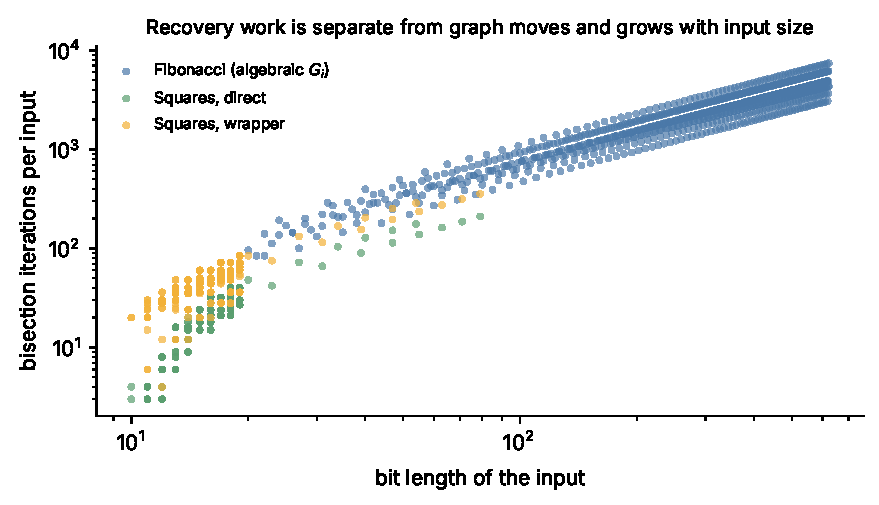
\includegraphics[width=.85\textwidth]{figures/fig2_cost.pdf}
\caption{Bisection iterations per input against input bit length, for $30\le k<900$ (Fibonacci) and a spread of $n$ up to $10^8$ (squares). Graph moves are at most $12$, $5$ and $8$ respectively; recovery work dominates.}
\end{figure}
Over $30\le k<900$ the Fibonacci selector uses a mean of \FibItersMean{} bisection iterations per input (maximum \FibItersMax), about \FibSlope{} iterations per input bit, against about \SqDSlope{} (direct) and \SqWSlope{} (wrapper) for squares, while using at most $12$ graph moves. The difference reflects the route length, the large intermediate states ($\sim F_k^{\,2}$--$F_k^{\,5}$) whose parameters must be re-derived at every step, and the exact radical comparisons. These are costs of the Python implementation in big-integer operations, not a formal complexity bound.

\section{The Generative Knowledge Audit}\label{sec:audit}
\paragraph{Method.} For each route class and each step, the label $N$ is evaluated at $26$ points of the class (exact integers). In order, we test whether $N$ is
\emph{constant}; a \emph{polynomial of degree $\le3$ in the current state $S$} (``local''); satisfies an \emph{algebraic relation $P(N,S)=0$ with $\deg_N,\deg_S\le2$} (``algebraic in $S$''); lies in the \emph{route-start field} (for Fibonacci, $\Q[x_0,L_k]$ with $L_k=\isqrt(5x_0^2\pm4)$; for squares, $\Q[n]$ with $n=\isqrt(x_0)$; for the wrapper, $\Q[m]$ with $m$ the state after its first move), with $x_0$-degree $\le9$ or polynomial degree $\le4$; or a polynomial in the destination state $S_{\rm after}$. A label in the first three classes is computable from the current state alone (``local'' and ``algebraic in $S$'' by a fixed-order root and exact division), with no recovery of route-start parameters. All fits are exact rational interpolation verified at all sample points.

\begin{table}[ht]\centering\small
\begin{tabular}{@{}lrrrrrrr@{}}\toprule & steps & const & local & alg.\ in $S$ & field & dest. only & not found\\\midrule
Fibonacci & 99 & 9 & 14 & 15 & 51 & 0 & 10\\
Squares, direct & 105 & 23 & 27 & 37 & 18 & 0 & 0\\
Squares, wrapper & 64 & 16 & 22 & 23 & 3 & 0 & 0\\
\bottomrule\end{tabular}

\caption{Classification of every route step. ``Field'': needs route-start parameters ($x_0$, $L_k$ or $n$). ``Not found'': in none of the above, within the stated vocabulary.}
\label{tab:audit}
\end{table}
\begin{figure}[ht]\centering
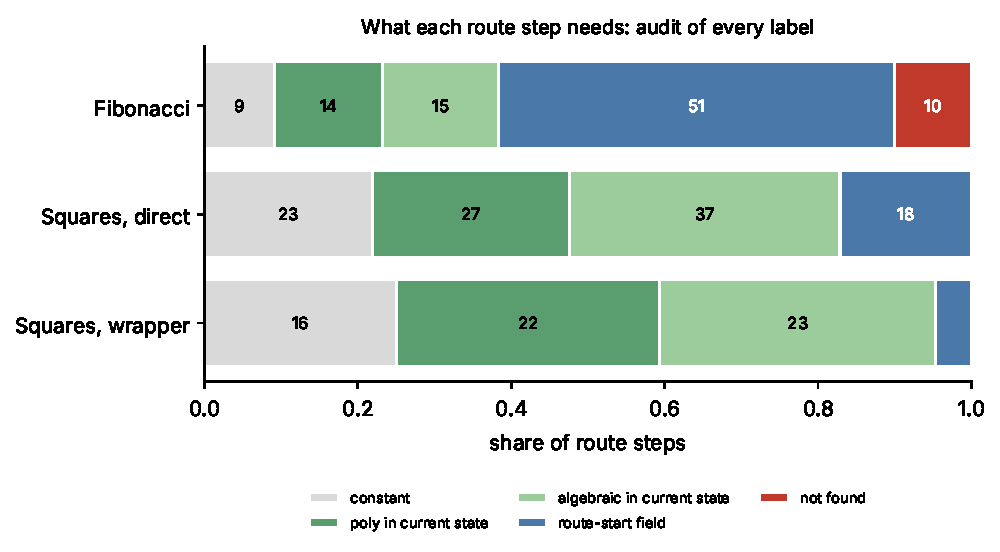
\includegraphics[width=.9\textwidth]{figures/fig1_audit.pdf}
\caption{Share of route steps by what their label needs.}
\end{figure}

\paragraph{Findings.}
(1)~For the squares selectors \SqDNoRec{} of \NSqD{} and \SqWNoRec{} of \NSqW{} labels are computable from the current state without recovery; no step is unexplained. (2)~For Fibonacci only \FibNoRec{} of \NFib{} are. Of the remaining labels, $51$ lie in $\Q[x_0,L_k]$ and in fact have $x_0$-degree at most $1$ (nine are $\alpha+\beta L_k$, forty-two are bilinear in $x_0$ and $L_k$): they are \emph{polynomial in the start value and the Cassini root}. (3)~The \emph{ten} labels not found in $\Q[x_0,L_k]$ (classes $1$ and $9$, Appendix) are exactly those that are odd in the half-index values $F_{h-1},F_h$ (for example $(2F_{h-1}+3F_h+1)/2$); they need the duplication relation $x_0=F_{2h+1}=F_h^2+F_{h+1}^2$ as a second quadratic, i.e.\ recovery of the half-index parameter. We do not claim they are impossible to express otherwise. (4)~Because the selector sees only the current state, the recovery functions $G_i$ are how it re-derives route-start parameters: the audit \emph{measures} how much of each route depends on that re-derivation.

\paragraph{Caveats.} The categories are verified at sample points, not proved as identities (they could be upgraded by the multiplication method of the Cassini ring; not done here). ``Algebraic in $S$'' records an existing relation of degree $\le(2,1)$ (here always of the shape $S=$ quadratic in $N$, i.e.\ labels like $\isqrt(S/c)-d$); the selectors as implemented do not use these shortcuts, and the shortcuts were not implemented as selectors.

\section{The knowledge ledger}\label{sec:ledger}
\begin{table}[ht]\centering\footnotesize
\begin{tabular}{@{}p{3.1cm}p{3.6cm}p{3.6cm}p{3.6cm}@{}}\toprule & Fibonacci & Squares, direct & Squares, wrapper\\\midrule
Membership & \texttt{isqrt} test: $5x^2+4$ or $5x^2-4$ a square & \texttt{isqrt} test: $x=n^2$ & \texttt{isqrt} test: $x=n^2$\\
Fixed-modulus dispatch & $(x \bmod 24,\ y \bmod 24)$, $y=(x+L_k)/2$ & $n \bmod 24$ & $n \bmod 24$ (class table inside U2-001)\\
Parameter recovery & algebraic state functions $G_i$ (with $\alpha_\varepsilon$), exact radical bisection & polynomial state functions, bisection & polynomial state functions (U2-001), bisection\\
Control states & 201 & 85 & 45\\
Route labels & 99 & 105 & 64\\
Moves (max) & 12 & 5 & 8\\
Target value formed at READY & yes & no (computable) & no (computable)\\
External information & none & none & none\\
\bottomrule\end{tabular}

\caption{Ledger for the three selectors. Control states are counted as $1+\sum(\text{steps}-1)$ over route classes and small-table paths (the convention of UNNS-U2-SQ). The Fibonacci figure of \FibQ{} comprises $87$ for the twelve route classes (the earlier ``99'' counted route \emph{labels}) and $113$ for the small-index table.}
\end{table}
Under the five-source schema of the review:
\begin{itemize}\setlength\itemsep{1pt}
\item \textbf{Reversible arithmetic} supplies legality (divisibility conditions, Lemma~1 of UNNS-U2-FP-SYM) and the existence of bounded routes, and, by the audit, the whole of the label for \FibNoRec/\NFib{} Fibonacci steps and for most steps of both square selectors.
\item \textbf{Membership} is supplied by the controller: $\isqrt$ tests ($5x^2\pm4$ for Fibonacci; $x=n^2$ for squares).
\item \textbf{Parameter recovery} is supplied by the controller: algebraic monotone state functions (with $\alpha_\varepsilon$) for Fibonacci, polynomial ones for squares. This is where Fibonacci differs most.
\item \textbf{Route knowledge} is supplied by the controller: the twelve precertified route classes, the residue dispatch mod $24$ (both families) and, for Fibonacci, a $28$-path small table.
\item \textbf{External information}: none. The selectors read only the current integer and the control state. All three can form their target value from the ready state with the same primitives; the Fibonacci selector does so explicitly.
\end{itemize}
\paragraph{Reading.} The contribution of the reversible arithmetic is real but is the \emph{geometry} of the graph (legal edges, short routes), not the identity of the next term. For squares the controller's algebraic knowledge is light and mostly polynomial. For Fibonacci it is heavier: the Cassini quadratic, the half-index relation and a larger recovery apparatus. The Fibonacci result is therefore \emph{autonomous bounded-route generation under a restricted arithmetic selector}.

\section{Consequences for the next families, including primes}
Any new sequence family should be accompanied by the same ledger. For primes the entries are sharp. The graph supplies local structure (neighbour rigidity, $\mathrm{Nbr}(p)=\{4p,(p+1)^2\}$); no membership test, parameter recovery or route family under R3$'$ and R4 has been constructed. Primality testing, factorisation and candidate search are excluded by the selector class, so any prime selector must put its knowledge into membership, recovery or route entries explicitly and without such search. We make \emph{no impossibility claim}: that no admissible prime-successor selector has been constructed is not a proof that none exists, and the absence of a closed form in our restricted vocabularies is not a theorem.

\section{Acceptance gates and unverified assumptions}
\begin{center}\small
\begin{tabular}{@{}p{3.0cm}p{9.5cm}@{}}\toprule
Gate & Evidence in this package\\\midrule
Mathematical & Lemma~\ref{lem:sign}; Theorem~\ref{thm:mono}; items R1, R2 (exact), R2n (numerical)\\
Domain & items R3, R4, R4a, R5, R7: accepted and refused inputs, dispatch, small table\\
Knowledge accounting & items R6, R8, R9: audit, costs, ledger (same rules applied to U2-SQ)\\
Reproducibility & deterministic report, source and input hashes, edge replay with an independent predicate, README \texttt{NOT\_RERUN}\\\bottomrule
\end{tabular}\end{center}
\paragraph{Unverified.} (i)~The route certificates are inherited and rest on SymPy, not a proof assistant. (ii)~Audit categories are verified at sample points only. (iii)~`Not found' is not necessity. (iv)~Costs are Python big-integer counts. (v)~Whether R3$'$ is the intended reading of Definition~2.1 is a decision of the programme, not a theorem. (vi)~No literature search for priority was carried out.

\begin{thebibliography}{9}
\bibitem{koshy} T.~Koshy, \emph{Fibonacci and Lucas Numbers with Applications}, Wiley, 2001.
\bibitem{sympy} A.~Meurer et al., SymPy: symbolic computing in Python, \emph{PeerJ Computer Science} \textbf{3}:e103 (2017).
\bibitem{fp} UNNS Research Collective, UNNS-U2-FP-SYM v001; UNNS-U2-FP v001; UNNS-U2-SQ v001 (all frozen).
\end{thebibliography}

\appendix
\section{Per-class audit of the Fibonacci routes}
\begin{center}\small\begin{tabular}{@{}rl@{}}\toprule $k\bmod 12$ & step categories (c const, l local, a algebraic in $S$, F route-start field, ? not found)\\\midrule
0 & \texttt{clFFFFac}\\
1 & \texttt{lF???F???a}\\
2 & \texttt{lFFFFFFa}\\
3 & \texttt{lFFFFala}\\
4 & \texttt{clFFa}\\
5 & \texttt{lFFFFFFFFa}\\
6 & \texttt{lFFFFFFa}\\
7 & \texttt{lFFacla}\\
8 & \texttt{lFFFFa}\\
9 & \texttt{lF????FFFa}\\
10 & \texttt{cclFFca}\\
11 & \texttt{lFFFFFFacFac}\\
\bottomrule\end{tabular}
\end{center}
Classes $1$ and $9$ contain all ten steps marked \texttt{?}.
\end{document}
